\section{Arithmetic and geometric operations.}
\begin{enumerate}[label=\emph{\alph*)}]
\item What is the min and max of the values of $img-green$? What is the mean? What is the standard deviation? How do you compute them? Provide code snippets in your report for these questions.

The results for each $img-green$ is summarized on table \ref{table:statistics}

\begin{table} [!htb]
\setlength{\tabcolsep}{2.7mm}
\centering
\begin{tabular}{lcccc}
\toprule
\textbf{Img. name}  & \textbf{max} & \textbf{min} & \textbf{mean} & \textbf{std. deviation}\\
\midrule
p0-2-b-0.jpg & 255 & 0 & 137.844325718 & 61.710497328 \\
p0-2-b-1.jpg & 255 & 0 & 198.553740686 & 76.377641762  \\
p0-2-b-2.jpg & 255 & 0 & 137.885818781 & 61.294456676 \\
p0-2-b-3.jpg & 255 & 0 & 138.209035652 & 77.913647393 \\
\bottomrule
\end{tabular}
\caption{Summary for image statistics}
\label{table:statistics}
\end{table}

The code snippet for this problem is relative small using python:

\begin{lstlisting}[language=python]
import numpy as np
def question_A(img):
	img_max = img.max() #image max
	img_min = img.min() #image min
	img_mean = img.sum()/(1. * img.shape[0] * img.shape[1]) #image mean
	img_std = np.std(img.ravel()) #image standard deviation
	print ('max:', img_max, 'min:', img_min, 'mean:', img_mean, 'std:', img_std)
\end{lstlisting}

\item Normalize the values of img-green. How the image looks like? Do you have an idea of what happened?

The results of the normalization are shown in figure \ref{fig:green-normalization}.

\begin{figure}[h!]
\centering
\begin{subfigure}{0.5\textwidth}
  \centering
  
\includegraphics[width=0.5\linewidth]{../output/p0-4-b-0.jpg}
  \caption{Output for $img-green$ of p0-1-0.jpg}
  \label{fig:sfig1}
\end{subfigure}%
\begin{subfigure}{0.5\textwidth}
  \centering
  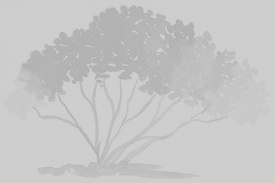
\includegraphics[width=0.5\linewidth]{../output/p0-4-b-1.jpg}
  \caption{Output for $img-green$ of  p0-1-1.jpg}
  \label{fig:sfig2}
\end{subfigure}
\begin{subfigure}{0.5\textwidth}
  \centering
  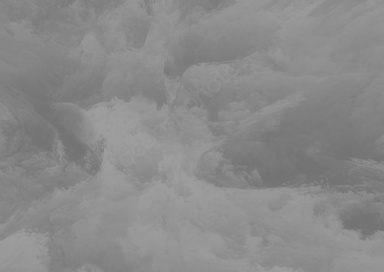
\includegraphics[width=0.5\linewidth]{../output/p0-4-b-2.jpg}
  \caption{Output for $img-green$ of p0-1-2.jpg}
  \label{fig:sfig3}
\end{subfigure}%
\begin{subfigure}{0.5\textwidth}
  \centering
  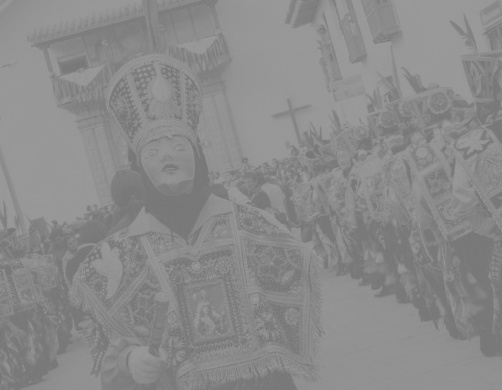
\includegraphics[width=0.5\linewidth]{../output/p0-4-b-3.jpg}
  \caption{Output for $img-green$ of p0-1-3.jpg}
  \label{fig:sfig4}
\end{subfigure}
\caption{Output images for question 4.b}
\label{fig:green-normalization}
\end{figure}

Comparing this images with the originals, it seems that a gray mask has been applied, this turns the image less visually-readable. The explanation for this effect can be done analysing the histograms that the images generate (figure \ref{fig:hist-normalization}). In the normalized image, the color are centered and go from a range of $[0, 255]$ to a smaller one, note that the shape of the histograms (visual relation between bins size) remains the same, hence, the normalization works as a operation that push the bins to the center values.


\begin{figure}[h!]
\centering
\begin{subfigure}{0.5\textwidth}
  \centering
  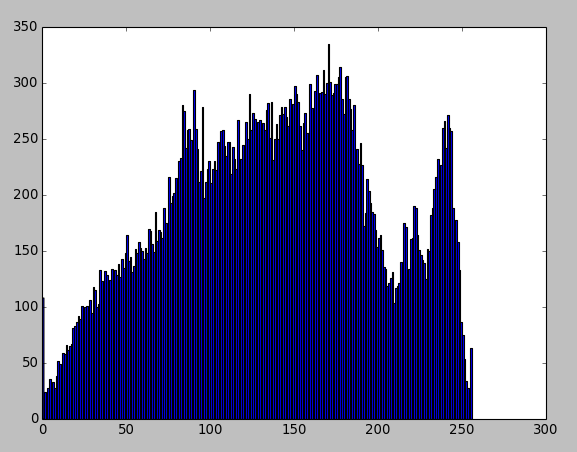
\includegraphics[width=0.5\linewidth]{../dbg/hist-original.png}
  \caption{Histogram for $img-green$ of p0-1-0.jpg}
\end{subfigure}%
\begin{subfigure}{0.5\textwidth}
  \centering
  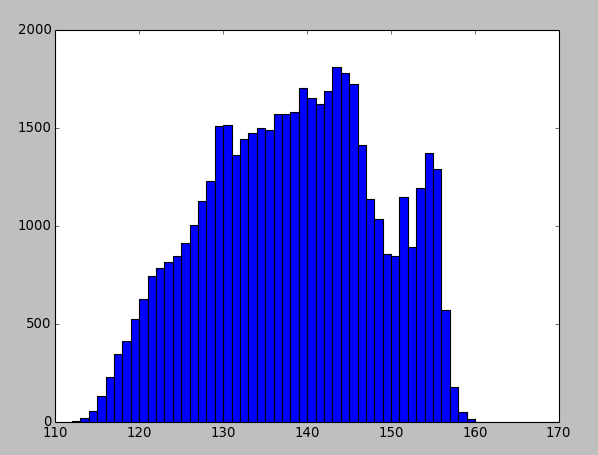
\includegraphics[width=0.5\linewidth]{../dbg/hist-normalized.png}
  \caption{Histogram for norm. $img-green$ of  p0-1-1.jpg}
\end{subfigure}
\caption{Histograms for $img-green$ and its normalizated image}
\label{fig:hist-normalization}
\end{figure}


\item Shift img-green to the left by 2 pixels. Store the resulting image in the output folder. Subtract the shifted version to the original, and save the difference image. Make sure that all the values you are saving are legal so you can see all the differences. What do the negative values mean? What do you see in the result?

The results for the shifted image, and the original image subtracted with the shifted are shown in figure \ref{fig:shifted-results}, the images shifted to left by two pixel present a black line which actually are the parts of the image that were replaced with 0 as part of the shifting. In the case of the subtracted image, an interesting effects accours: it presents approximation of the edges from the original images. This is really interesting and the min, max, mean and standard deviation (table \ref{table:statistics-shifted}) of the subtracted image can give an intuition of this effect.

Comparing the image statistics, we can see a big effect in the mean: it has decreased widely, since in RGB system a value 0 is equal to black, all the pixel that has negative value are represented with black, and they may represent no-edges, this is because edges are consider as elements with high frequency, thus, when subtracting with an adjacent pixel (shifted image) its value is usually bigger and the result is positive (not black).


\begin{table} [!htb]
\setlength{\tabcolsep}{2.7mm}
\centering
\begin{tabular}{lcccc}
\toprule
\textbf{Img. name}  & \textbf{max} & \textbf{min} & \textbf{mean} & \textbf{std. deviation}\\
\midrule
p0-2-b-0.jpg & 232 & -211 & 1.00700073692 & 46.3247164932 \\
p0-2-b-1.jpg & 255 & -253 & 1.83093889717 & 44.5053782822 \\
p0-2-b-2.jpg & 216 & -168 & 0.64044309129 & 19.2998234779 \\
p0-2-b-3.jpg & 239 & -234 & 0.60832567167 & 43.4115692626 \\
\bottomrule
\end{tabular}
\caption{Summary for image statistics}
\label{table:statistics-shifted}
\end{table}

\begin{figure}[h!]
\centering
\begin{subfigure}{0.5\textwidth}
  \centering
  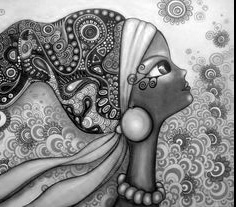
\includegraphics[width=0.5\linewidth]{../output/p0-4-c-0.jpg}
  \caption{Shifted image for input p0-1-0.jpg}
\end{subfigure}%
\begin{subfigure}{0.5\textwidth}
  \centering
  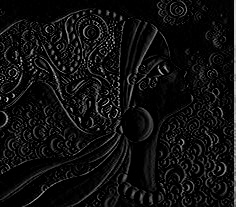
\includegraphics[width=0.5\linewidth]{../output/p0-4-c-1.jpg}
  \caption{Original subtracted with shifted image for p0-1-0.jpg}
\end{subfigure}
\begin{subfigure}{0.5\textwidth}
  \centering
  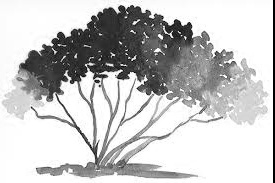
\includegraphics[width=0.5\linewidth]{../output/p0-4-c-2.jpg}
  \caption{Shifted image for input p0-1-1.jpg}
\end{subfigure}%
\begin{subfigure}{0.5\textwidth}
  \centering
  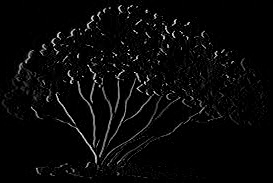
\includegraphics[width=0.5\linewidth]{../output/p0-4-c-3.jpg}
  \caption{Original subtracted with shifted image for p0-1-1.jpg}
\end{subfigure}

\begin{subfigure}{0.5\textwidth}
  \centering
  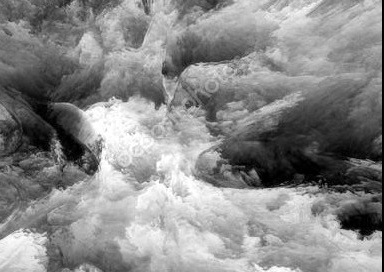
\includegraphics[width=0.5\linewidth]{../output/p0-4-c-4.jpg}
  \caption{Shifted image for input p0-1-2.jpg}
\end{subfigure}%
\begin{subfigure}{0.5\textwidth}
  \centering
  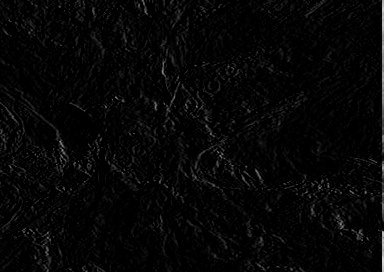
\includegraphics[width=0.5\linewidth]{../output/p0-4-c-5.jpg}
  \caption{Original subtracted with shifted image for p0-1-2.jpg}
\end{subfigure}
\begin{subfigure}{0.5\textwidth}
  \centering
  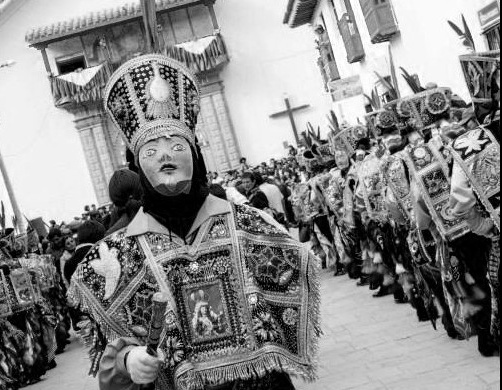
\includegraphics[width=0.5\linewidth]{../output/p0-4-c-6.jpg}
  \caption{Shifted image for input p0-1-3.jpg}
\end{subfigure}%
\begin{subfigure}{0.5\textwidth}
  \centering
  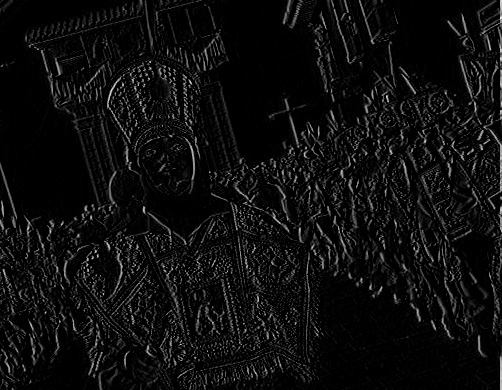
\includegraphics[width=0.5\linewidth]{../output/p0-4-c-7.jpg}
  \caption{Original subtracted with shifted image for p0-1-3.jpg}
\end{subfigure}

\caption{Output images for question 4.c}
\label{fig:shifted-results}
\end{figure}
\end{enumerate}
